\subsection{Auswertung}
Bei der Analyse des vorgegebenen Pulvers mittels Debye Scherrer Verfahren ergab sich das Diffraktogramm in Abb. \ref{fig:diffr_pulver}.
Zum Vergleich sind Diffraktogramme von Silicium und Germanium (Abb. \ref{fig:diffr_sil_sim} und Abb. \ref{fig:diffr_ger_sim}) simuliert worden. Man sieht sofort, dass das Diffraktogramm von Silicium mit dem der untersuchten Probe sehr gut �bereinstimmt. Daneben stellt man einen Offset der simulierten Daten zu den gemessenen fest. Um diesen Offset zu bestimmen, wurde an alle drei Datens�tze ein Multivoigt gefittet. Die Voigtverteilung wird dabei numerisch approximiert, wobei die in Python bereits implementierte Voigt-Verteilung aus der Bibliothek "`lmfit"' verwendet wird. Der Fit an die Messdaten passt mit einem reduzierten Chiquadrat von 22,335 relativ gut, wenn man beachtet, dass auch bei kleineren Zahlraten ein Fehler von $\sqrt{N}$ verwendet wurde. Erstaunlicherweise passen die Fits, bei einem Fehler von $\sqrt{N}$, eher schlecht an die simulierten Daten. Man sieht aber, dass die Maxima gut getroffen werden, was in diesem Versuchsteil das wichtigste Kriterium f�r die Auswertung ist. Es ergeben sich reduzierte Chiquadrate von 562 und 19989, sodass diese Fits nicht als besonders gut betrachtet werden k�nnen. Wie die Fits in der N�he einzelner Peaks aussehen, kann im Anhang nachvollzogen werden.
\begin{sidewaysfigure}
\centering
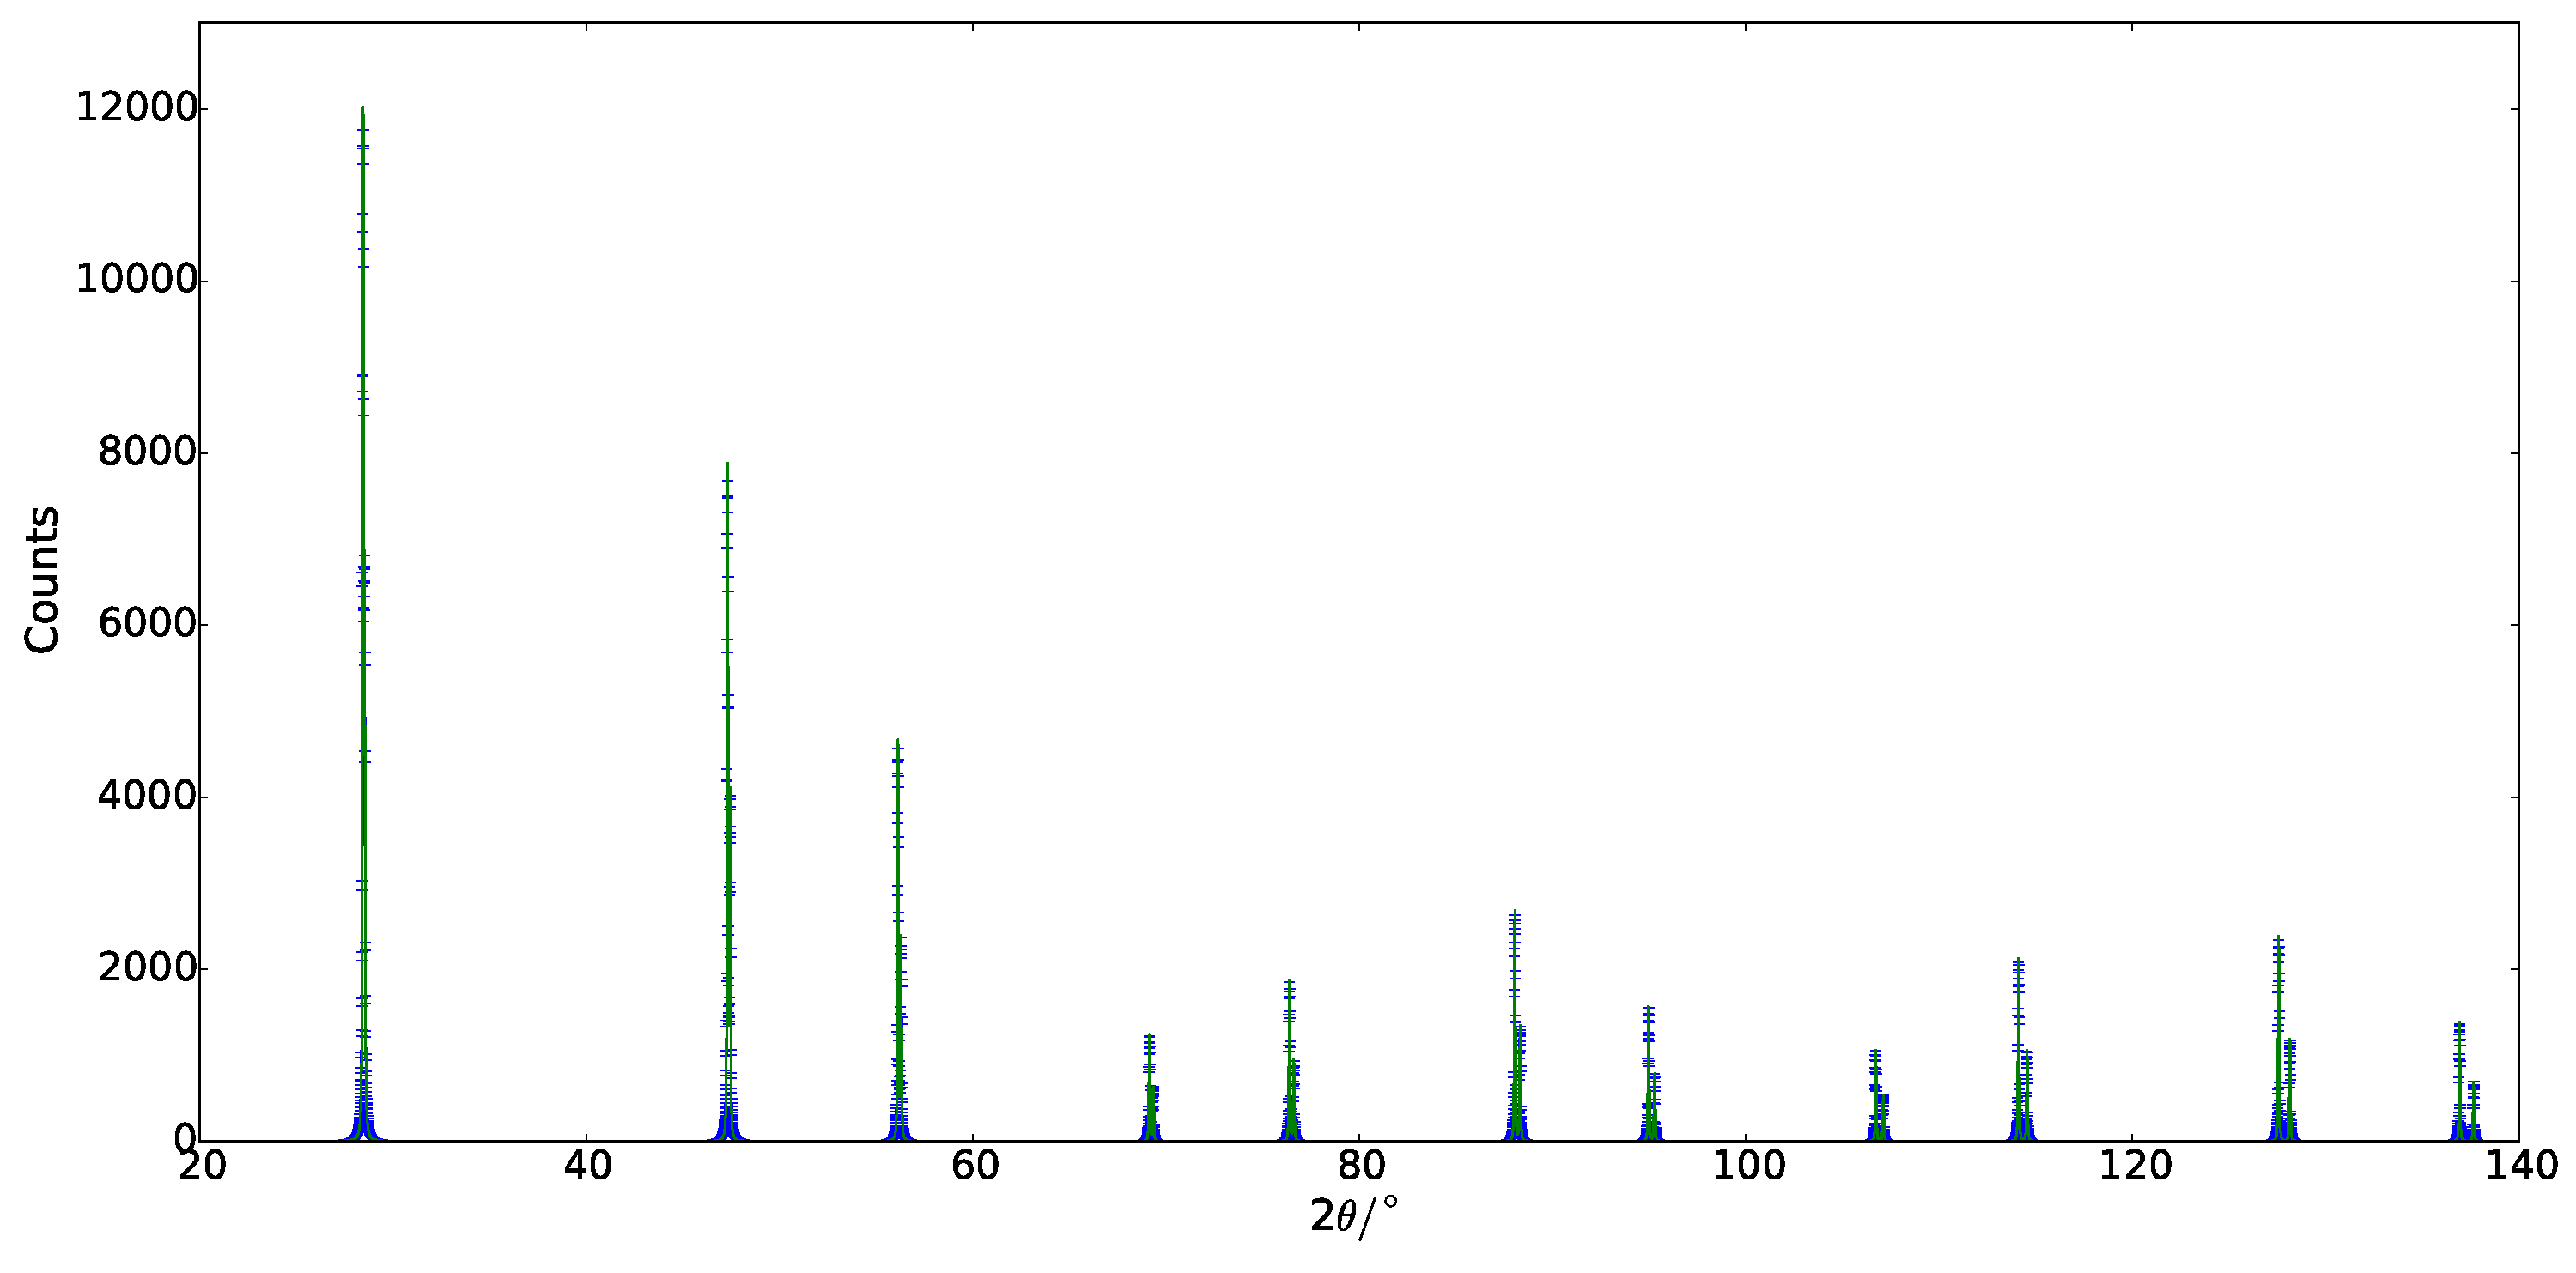
\includegraphics[width = 1.0\textwidth, height = 0.7\textwidth]{messung_pulver_ges}
\caption{Diffraktogramm der Pulverprobe}
\label{fig:diffr_pulver}
\end{sidewaysfigure}
\begin{sidewaysfigure}
\centering
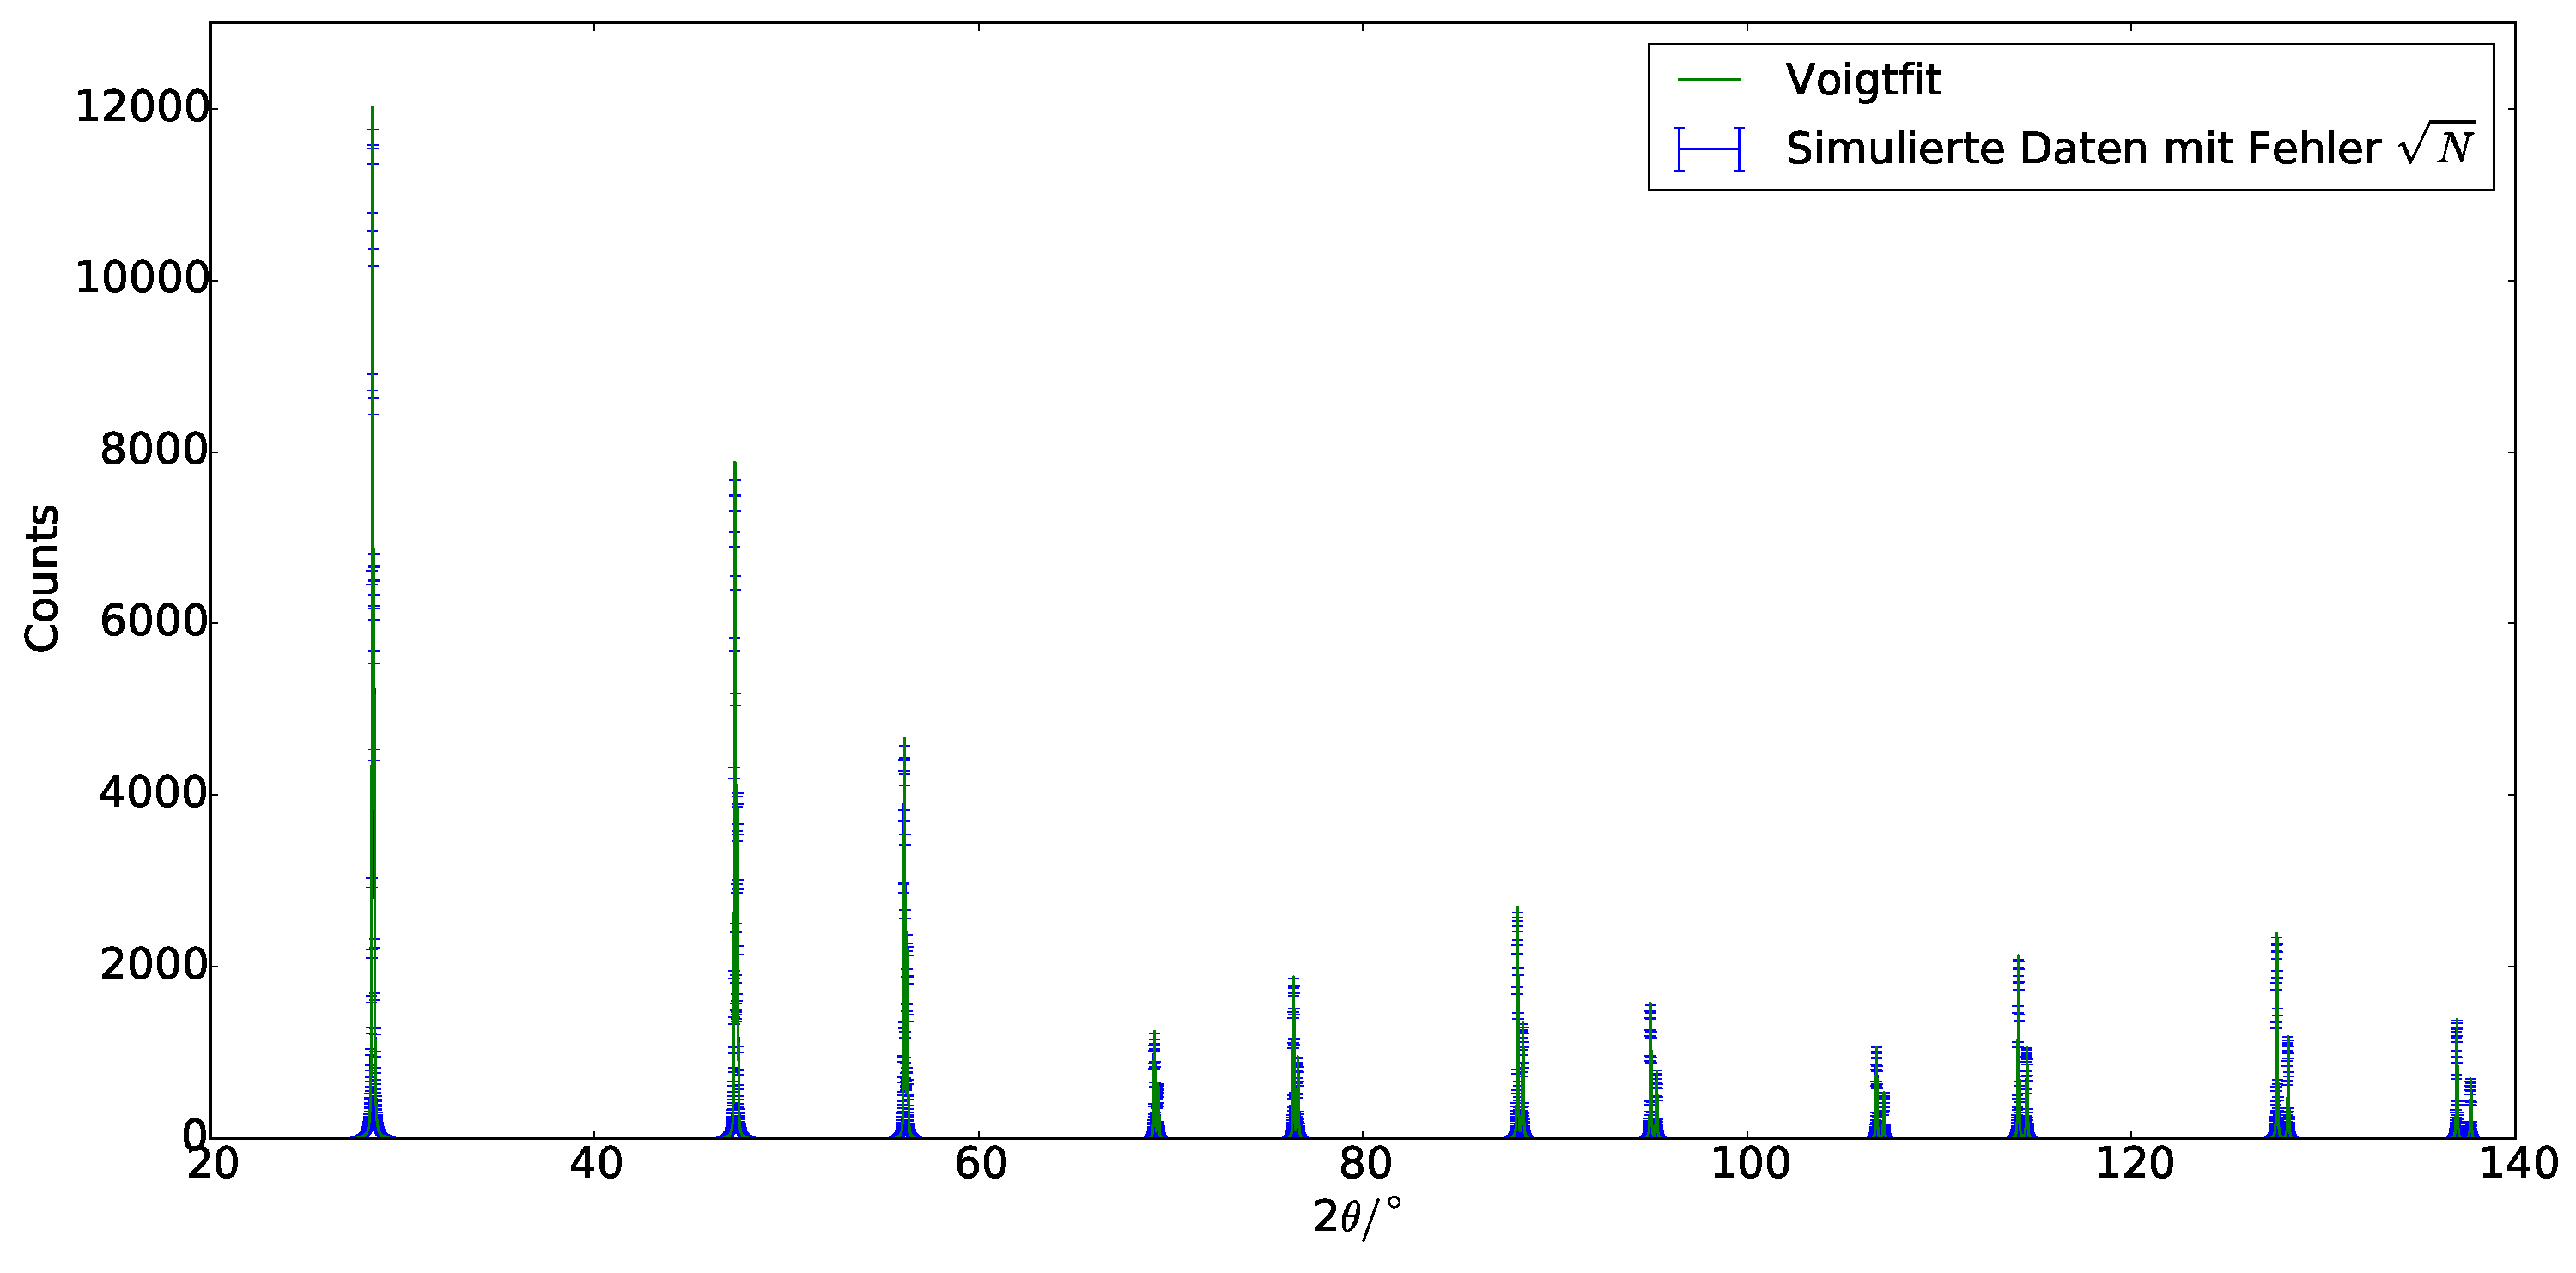
\includegraphics[width = 1.0\textwidth, height = 0.7\textwidth]{Simulation_Siliciumpulver_ges}
\caption{Diffraktogramm der Siliciumsimulation}
\label{fig:diffr_sil_sim}
\end{sidewaysfigure}
\begin{sidewaysfigure}
\centering
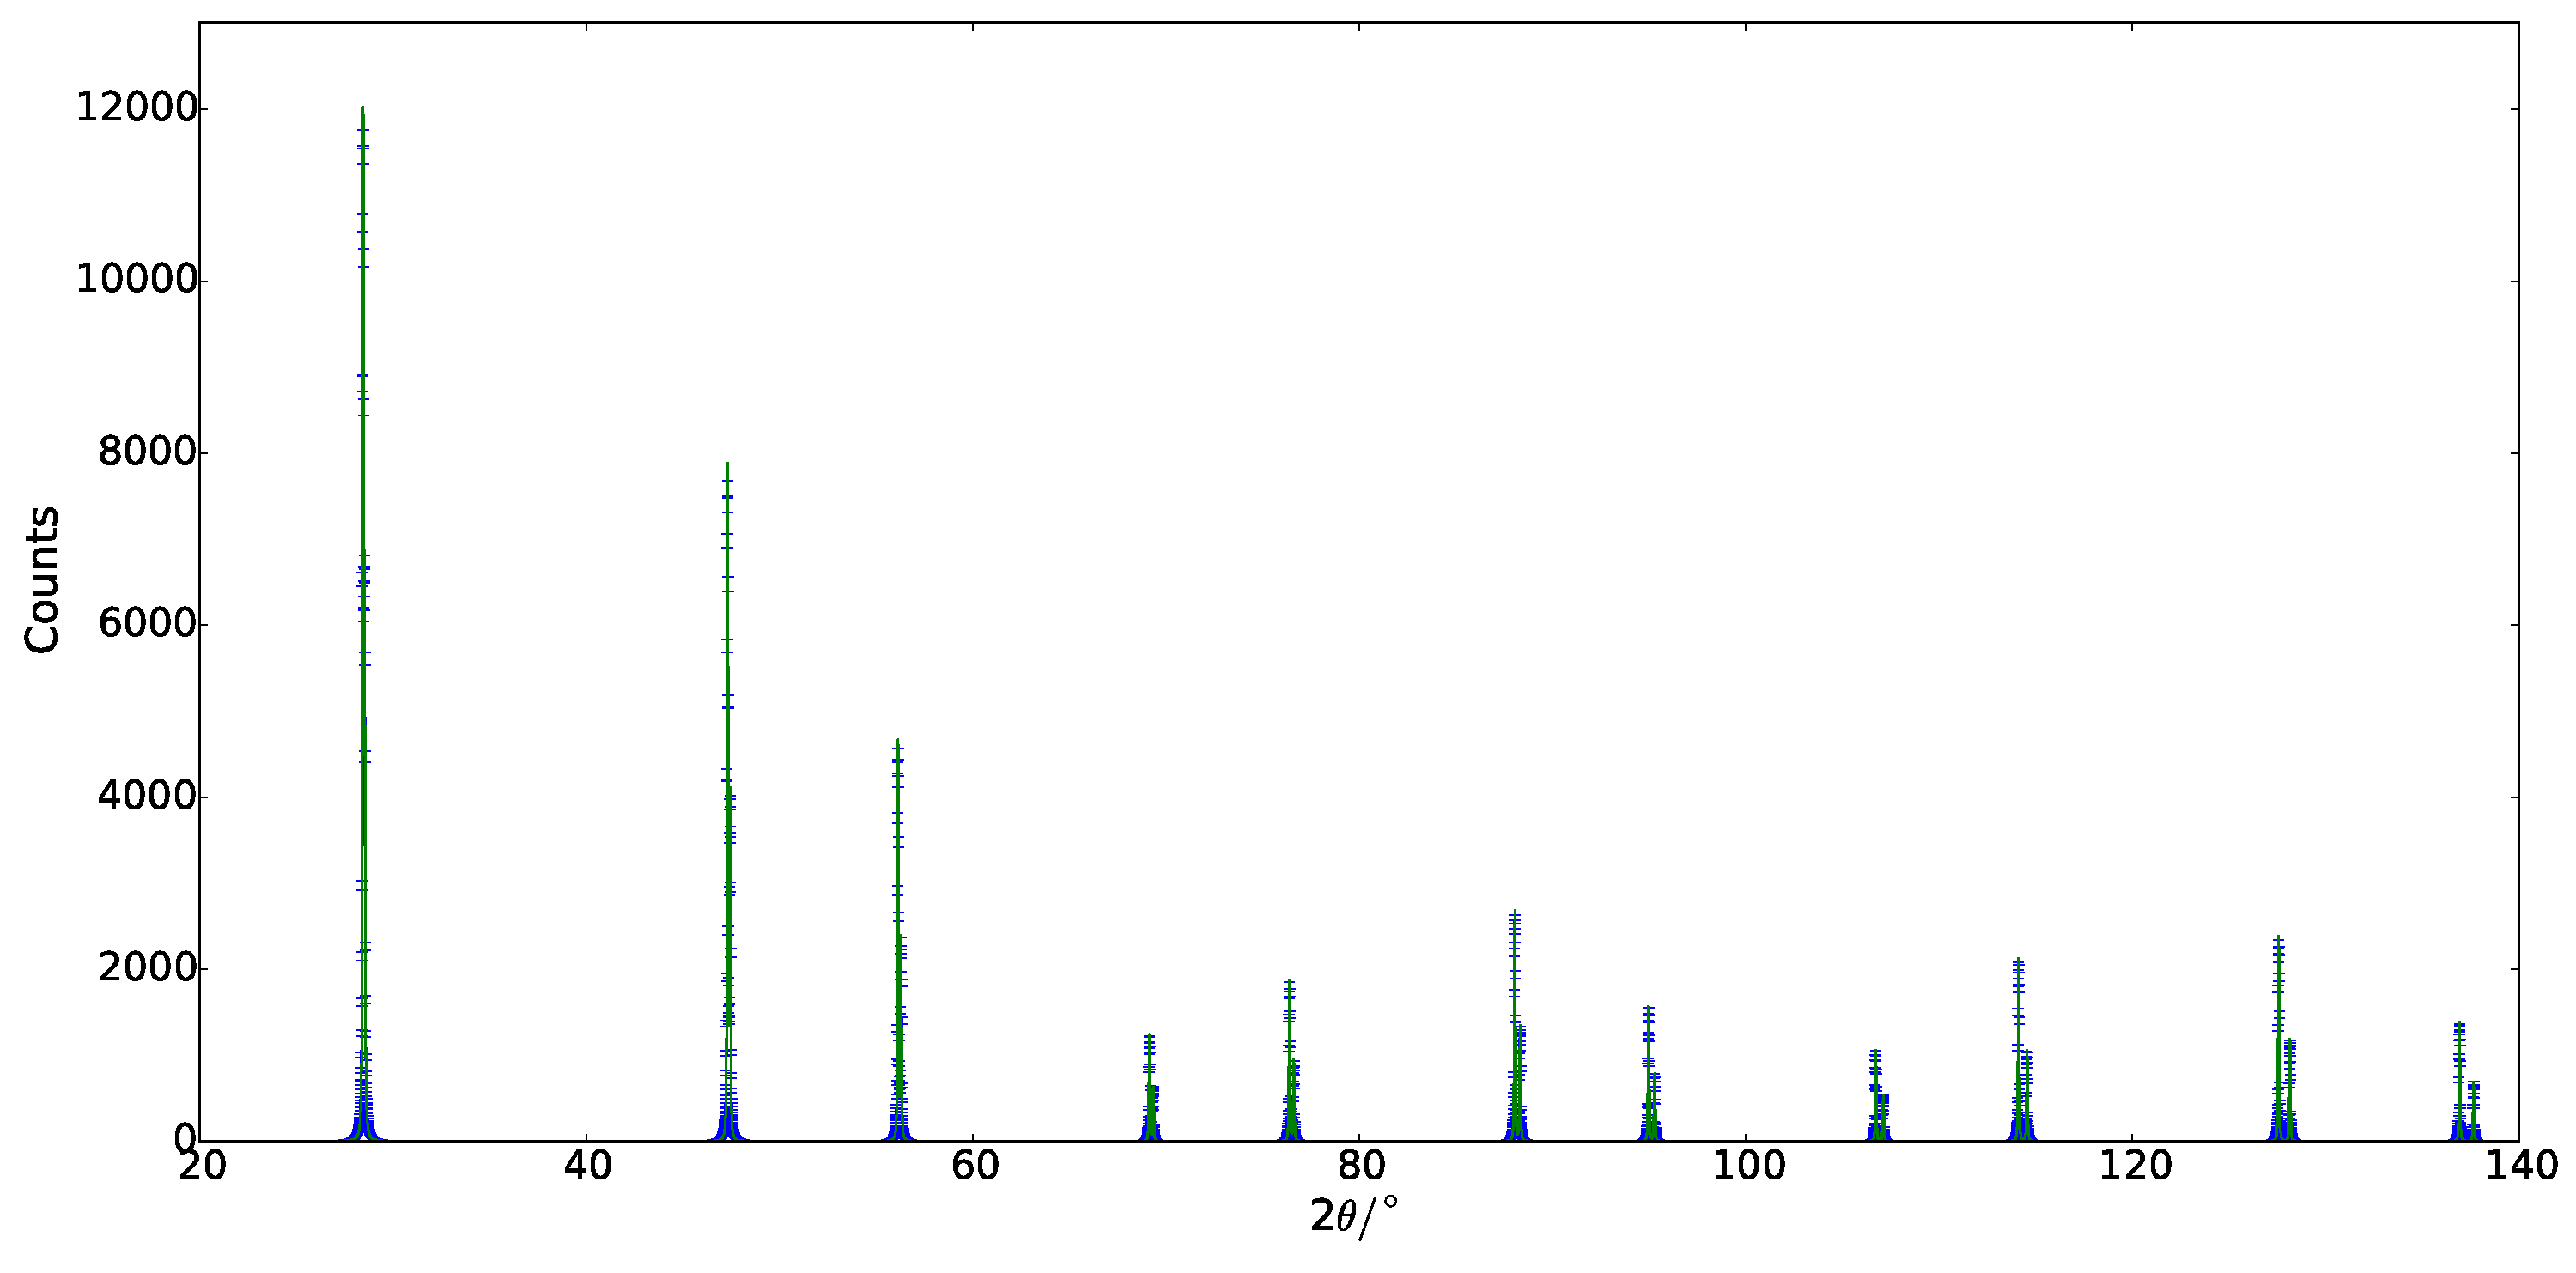
\includegraphics[width = 1.0\textwidth, height = 0.7\textwidth]{messung_pulver_ges}
\caption{Diffraktogramm der Germaniumsimulation}
\label{fig:diffr_ger_sim}
\end{sidewaysfigure}